\documentclass[10pt, twoside, a4paper]{article}
\usepackage[italian]{babel}
%\usepackage[utf8]{inputenc}
\usepackage{fullpage}
\usepackage{graphicx}
%\usepackage{booktabs}
%\usepackage{wrapfig}
%\usepackage{sidecap}
%\usepackage[small]{caption}
\usepackage{gchords}			%serve per scrivere gli accordi
\setlength{\parindent}{0in}	%serve per togliere l'indentazione della prima riga
\usepackage[usenames,dvipsnames,svgnames,table]{xcolor}	%serve per utilizzare i colori \textcolor{blue}{}

\begin{document}

\begin{center}

	\hrule \vspace{0.2cm}
     	\textsc{\LARGE Mi piaccion le sbarbine}
	\vspace{0.2cm} \hrule \vspace{0.2cm}
      	{\large Skiantos}

%	{\begin{abstract}
%	blablalba
%	 \end{abstract}}

\chords{\chord{t}{o,p2,p2,p1,o,o}{E}
		\chord{{3~}}{p1,p3,p3,p2,p1,p1}{G}
		\chord{{5~}}{p1,p3,p3,p2,p1,p1}{A}
		\chord{{7~}}{p1,p3,p3,p2,p1,p1}{B}}

\end{center}

Mi \upchord{E}piaccion le sbarbine...i \\
Mi \upchord{A}piaccion le sbarbine...i \\
Mi \upchord{B}piaccion le sbarbine...i \\

\begin{figure}[ht!]
	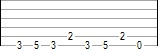
\includegraphics{images/temp.jpg}
\end{figure}

Non \upchord{G}posso farci \upchord{A}niente			\hfill	\upchord{B}Mi piaccion le sbar\upchord{E}bine \\ 
Mi sento deficiente				\hfill	Yeah yeah yeah... \\
Lo so che non conviene			\hfill	Mi piaccion le sbarbine \\
Ma poi chi si trattiene			\hfill	Mi piaccion le sbarbine \\

Quelle alte un metro e ottanta	\hfill	Yeah yeah yeah \\
Quelle basse uno e cinquanta		\hfill	Mi piaccion le sbarbine \\
Non esiste divisione				\hfill	No no no \\
Quel che conta è il calore...		\hfill	Mi piaccion le sbarbine \\

Le sbarbine sono bionde			\hfill	Le sbarbine sono more \\
Le sbarbine sono tante			\hfill	Le sbarbine in amore... \\

\begin{figure}[ht!]
	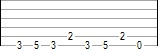
\includegraphics{images/temp.jpg}
\end{figure}

Mi \upchord{G}piaccion le sbar\upchord{A}bine			\hfill	\upchord{B}Yeah yeah ye\upchord{E}ah... \\
Anche se mi fan soffrire			\hfill	Mi piaccion le sbarbine \\
non c'ho mai niente da dire		\hfill	Mi piaccion le sbarbine \\
quel che voglio è solo amore		\hfill	Yeah yeah yeah...\\

Sono un tipo senza storia		\hfill	Mi piaccion le sbarbine \\
M'han fregato la memoria			\hfill	Mi piaccion le sbarbine \\
Ma l'amore di una sbarba			\hfill	Yeah yeah yeah... \\
Mi fa andare giu' di testa		\hfill	Mi piaccion le sbarbine \\

Le sbarbine sono bionde			\hfill	Le sbarbine sono more \\
Le sbarbine sono tante			\hfill	Le sbarbine in amore... \\

\begin{figure}[ht!]
	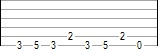
\includegraphics{images/temp.jpg}
\end{figure}

Le sbar\upchord{G}bine son car\upchord{A}ine			\hfill	\upchord{B}Mi piaccion le sbar\upchord{E}bine \\
Le sbarbine c'hanno gli occhi		\hfill	Yeah yeah yeah... \\
Le sbarbine con i tacchi			\hfill	Mi piaccion le sbarbine \\
Mi mandano nei matti				\hfill	Mi piaccion le sbarbine \\

Mi piaccion le sbarbine			\hfill	Yeah yeah yeah... \\
Lo so che non conviene			\hfill	No no no... \\
Mi piaccion le sbarbine			\hfill	Mi piaccion le sbarbine \\
Io voglio starci assieme			\hfill	Mi piaccion le sbarbine \\

Le sbarbine sono bionde			\hfill	Le sbarbine sono more \\
Le sbarbine sono tante			\hfill	Le sbarbine in amore... \\

\begin{figure}[ht!]
	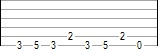
\includegraphics{images/temp.jpg}
\end{figure}

Yesss..!

\end{document}
